\documentclass[]{article}
\usepackage{lmodern}
\usepackage{amssymb,amsmath}
\usepackage{ifxetex,ifluatex}
\usepackage{fixltx2e} % provides \textsubscript
\ifnum 0\ifxetex 1\fi\ifluatex 1\fi=0 % if pdftex
  \usepackage[T1]{fontenc}
  \usepackage[utf8]{inputenc}
\else % if luatex or xelatex
  \ifxetex
    \usepackage{mathspec}
  \else
    \usepackage{fontspec}
  \fi
  \defaultfontfeatures{Ligatures=TeX,Scale=MatchLowercase}
\fi
% use upquote if available, for straight quotes in verbatim environments
\IfFileExists{upquote.sty}{\usepackage{upquote}}{}
% use microtype if available
\IfFileExists{microtype.sty}{%
\usepackage{microtype}
\UseMicrotypeSet[protrusion]{basicmath} % disable protrusion for tt fonts
}{}
\usepackage[margin=1in]{geometry}
\usepackage{hyperref}
\hypersetup{unicode=true,
            pdfborder={0 0 0},
            breaklinks=true}
\urlstyle{same}  % don't use monospace font for urls
\usepackage{color}
\usepackage{fancyvrb}
\newcommand{\VerbBar}{|}
\newcommand{\VERB}{\Verb[commandchars=\\\{\}]}
\DefineVerbatimEnvironment{Highlighting}{Verbatim}{commandchars=\\\{\}}
% Add ',fontsize=\small' for more characters per line
\usepackage{framed}
\definecolor{shadecolor}{RGB}{248,248,248}
\newenvironment{Shaded}{\begin{snugshade}}{\end{snugshade}}
\newcommand{\KeywordTok}[1]{\textcolor[rgb]{0.13,0.29,0.53}{\textbf{#1}}}
\newcommand{\DataTypeTok}[1]{\textcolor[rgb]{0.13,0.29,0.53}{#1}}
\newcommand{\DecValTok}[1]{\textcolor[rgb]{0.00,0.00,0.81}{#1}}
\newcommand{\BaseNTok}[1]{\textcolor[rgb]{0.00,0.00,0.81}{#1}}
\newcommand{\FloatTok}[1]{\textcolor[rgb]{0.00,0.00,0.81}{#1}}
\newcommand{\ConstantTok}[1]{\textcolor[rgb]{0.00,0.00,0.00}{#1}}
\newcommand{\CharTok}[1]{\textcolor[rgb]{0.31,0.60,0.02}{#1}}
\newcommand{\SpecialCharTok}[1]{\textcolor[rgb]{0.00,0.00,0.00}{#1}}
\newcommand{\StringTok}[1]{\textcolor[rgb]{0.31,0.60,0.02}{#1}}
\newcommand{\VerbatimStringTok}[1]{\textcolor[rgb]{0.31,0.60,0.02}{#1}}
\newcommand{\SpecialStringTok}[1]{\textcolor[rgb]{0.31,0.60,0.02}{#1}}
\newcommand{\ImportTok}[1]{#1}
\newcommand{\CommentTok}[1]{\textcolor[rgb]{0.56,0.35,0.01}{\textit{#1}}}
\newcommand{\DocumentationTok}[1]{\textcolor[rgb]{0.56,0.35,0.01}{\textbf{\textit{#1}}}}
\newcommand{\AnnotationTok}[1]{\textcolor[rgb]{0.56,0.35,0.01}{\textbf{\textit{#1}}}}
\newcommand{\CommentVarTok}[1]{\textcolor[rgb]{0.56,0.35,0.01}{\textbf{\textit{#1}}}}
\newcommand{\OtherTok}[1]{\textcolor[rgb]{0.56,0.35,0.01}{#1}}
\newcommand{\FunctionTok}[1]{\textcolor[rgb]{0.00,0.00,0.00}{#1}}
\newcommand{\VariableTok}[1]{\textcolor[rgb]{0.00,0.00,0.00}{#1}}
\newcommand{\ControlFlowTok}[1]{\textcolor[rgb]{0.13,0.29,0.53}{\textbf{#1}}}
\newcommand{\OperatorTok}[1]{\textcolor[rgb]{0.81,0.36,0.00}{\textbf{#1}}}
\newcommand{\BuiltInTok}[1]{#1}
\newcommand{\ExtensionTok}[1]{#1}
\newcommand{\PreprocessorTok}[1]{\textcolor[rgb]{0.56,0.35,0.01}{\textit{#1}}}
\newcommand{\AttributeTok}[1]{\textcolor[rgb]{0.77,0.63,0.00}{#1}}
\newcommand{\RegionMarkerTok}[1]{#1}
\newcommand{\InformationTok}[1]{\textcolor[rgb]{0.56,0.35,0.01}{\textbf{\textit{#1}}}}
\newcommand{\WarningTok}[1]{\textcolor[rgb]{0.56,0.35,0.01}{\textbf{\textit{#1}}}}
\newcommand{\AlertTok}[1]{\textcolor[rgb]{0.94,0.16,0.16}{#1}}
\newcommand{\ErrorTok}[1]{\textcolor[rgb]{0.64,0.00,0.00}{\textbf{#1}}}
\newcommand{\NormalTok}[1]{#1}
\usepackage{graphicx,grffile}
\makeatletter
\def\maxwidth{\ifdim\Gin@nat@width>\linewidth\linewidth\else\Gin@nat@width\fi}
\def\maxheight{\ifdim\Gin@nat@height>\textheight\textheight\else\Gin@nat@height\fi}
\makeatother
% Scale images if necessary, so that they will not overflow the page
% margins by default, and it is still possible to overwrite the defaults
% using explicit options in \includegraphics[width, height, ...]{}
\setkeys{Gin}{width=\maxwidth,height=\maxheight,keepaspectratio}
\IfFileExists{parskip.sty}{%
\usepackage{parskip}
}{% else
\setlength{\parindent}{0pt}
\setlength{\parskip}{6pt plus 2pt minus 1pt}
}
\setlength{\emergencystretch}{3em}  % prevent overfull lines
\providecommand{\tightlist}{%
  \setlength{\itemsep}{0pt}\setlength{\parskip}{0pt}}
\setcounter{secnumdepth}{0}
% Redefines (sub)paragraphs to behave more like sections
\ifx\paragraph\undefined\else
\let\oldparagraph\paragraph
\renewcommand{\paragraph}[1]{\oldparagraph{#1}\mbox{}}
\fi
\ifx\subparagraph\undefined\else
\let\oldsubparagraph\subparagraph
\renewcommand{\subparagraph}[1]{\oldsubparagraph{#1}\mbox{}}
\fi

%%% Use protect on footnotes to avoid problems with footnotes in titles
\let\rmarkdownfootnote\footnote%
\def\footnote{\protect\rmarkdownfootnote}

%%% Change title format to be more compact
\usepackage{titling}

% Create subtitle command for use in maketitle
\providecommand{\subtitle}[1]{
  \posttitle{
    \begin{center}\large#1\end{center}
    }
}

\setlength{\droptitle}{-2em}

  \title{}
    \pretitle{\vspace{\droptitle}}
  \posttitle{}
    \author{}
    \preauthor{}\postauthor{}
    \date{}
    \predate{}\postdate{}
  

\begin{document}

\begin{center}\rule{0.5\linewidth}{\linethickness}\end{center}

title: ``Advanced Bioinformatics 2019 assessment'' author: ``Candidate
number 8941'' date: ``15/06/2019'' output: html\_document

\subsection{Task 1}\label{task-1}

\begin{Shaded}
\begin{Highlighting}[]
\KeywordTok{sum}\NormalTok{(}\DecValTok{5}\OperatorTok{:}\DecValTok{55}\NormalTok{)}
\end{Highlighting}
\end{Shaded}

\begin{verbatim}
## [1] 1530
\end{verbatim}

\subsection{Task 2}\label{task-2}

\begin{Shaded}
\begin{Highlighting}[]
\NormalTok{n=}\DecValTok{10}
\NormalTok{sumfun<-}\StringTok{ }\KeywordTok{sum}\NormalTok{(}\DecValTok{5}\OperatorTok{:}\NormalTok{n)}
\NormalTok{sumfun}
\end{Highlighting}
\end{Shaded}

\begin{verbatim}
## [1] 45
\end{verbatim}

\begin{Shaded}
\begin{Highlighting}[]
\NormalTok{n=}\DecValTok{20}
\NormalTok{sumfun<-}\StringTok{ }\KeywordTok{sum}\NormalTok{(}\DecValTok{5}\OperatorTok{:}\NormalTok{n)}
\NormalTok{sumfun}
\end{Highlighting}
\end{Shaded}

\begin{verbatim}
## [1] 200
\end{verbatim}

\begin{Shaded}
\begin{Highlighting}[]
\NormalTok{n=}\DecValTok{100}
\NormalTok{sumfun<-}\StringTok{ }\KeywordTok{sum}\NormalTok{(}\DecValTok{5}\OperatorTok{:}\NormalTok{n)}
\NormalTok{sumfun}
\end{Highlighting}
\end{Shaded}

\begin{verbatim}
## [1] 5040
\end{verbatim}

\subsection{Task 3}\label{task-3}

\begin{Shaded}
\begin{Highlighting}[]
\NormalTok{Fibonacci <-}\StringTok{ }\KeywordTok{numeric}\NormalTok{(}\DecValTok{12}\NormalTok{)}
\NormalTok{Fibonacci[}\DecValTok{1}\NormalTok{] <-}\StringTok{ }\NormalTok{Fibonacci[}\DecValTok{2}\NormalTok{] <-}\StringTok{ }\DecValTok{1}
\ControlFlowTok{for}\NormalTok{ (i }\ControlFlowTok{in} \DecValTok{3}\OperatorTok{:}\DecValTok{12}\NormalTok{) Fibonacci[i] <-}\StringTok{ }\NormalTok{Fibonacci[i}\OperatorTok{-}\DecValTok{2}\NormalTok{] }\OperatorTok{+}\StringTok{ }\NormalTok{Fibonacci[i}\OperatorTok{-}\DecValTok{1}\NormalTok{]}
\KeywordTok{print}\NormalTok{(Fibonacci)}
\end{Highlighting}
\end{Shaded}

\begin{verbatim}
##  [1]   1   1   2   3   5   8  13  21  34  55  89 144
\end{verbatim}

\subsection{Task 4}\label{task-4}

\begin{Shaded}
\begin{Highlighting}[]
\KeywordTok{library}\NormalTok{(ggplot2)}
\KeywordTok{str}\NormalTok{(mtcars)}
\end{Highlighting}
\end{Shaded}

\begin{verbatim}
## 'data.frame':    32 obs. of  11 variables:
##  $ mpg : num  21 21 22.8 21.4 18.7 18.1 14.3 24.4 22.8 19.2 ...
##  $ cyl : num  6 6 4 6 8 6 8 4 4 6 ...
##  $ disp: num  160 160 108 258 360 ...
##  $ hp  : num  110 110 93 110 175 105 245 62 95 123 ...
##  $ drat: num  3.9 3.9 3.85 3.08 3.15 2.76 3.21 3.69 3.92 3.92 ...
##  $ wt  : num  2.62 2.88 2.32 3.21 3.44 ...
##  $ qsec: num  16.5 17 18.6 19.4 17 ...
##  $ vs  : num  0 0 1 1 0 1 0 1 1 1 ...
##  $ am  : num  1 1 1 0 0 0 0 0 0 0 ...
##  $ gear: num  4 4 4 3 3 3 3 4 4 4 ...
##  $ carb: num  4 4 1 1 2 1 4 2 2 4 ...
\end{verbatim}

\begin{Shaded}
\begin{Highlighting}[]
\KeywordTok{ggplot}\NormalTok{(mtcars, }\KeywordTok{aes}\NormalTok{(}\DataTypeTok{x =} \KeywordTok{as.factor}\NormalTok{(gear), }\DataTypeTok{y =}\NormalTok{ mpg, }\DataTypeTok{fill =}\NormalTok{ gear))}\OperatorTok{+}
\StringTok{  }\KeywordTok{geom_point}\NormalTok{()}\OperatorTok{+}
\StringTok{  }\KeywordTok{geom_boxplot}\NormalTok{()}\OperatorTok{+}
\StringTok{  }\KeywordTok{labs}\NormalTok{(}\DataTypeTok{x=}\StringTok{'number of gears'}\NormalTok{, }\DataTypeTok{y=}\StringTok{'miles per gallon'}\NormalTok{, }\DataTypeTok{title=}\StringTok{'mtcars box plot'}\NormalTok{)}
\end{Highlighting}
\end{Shaded}

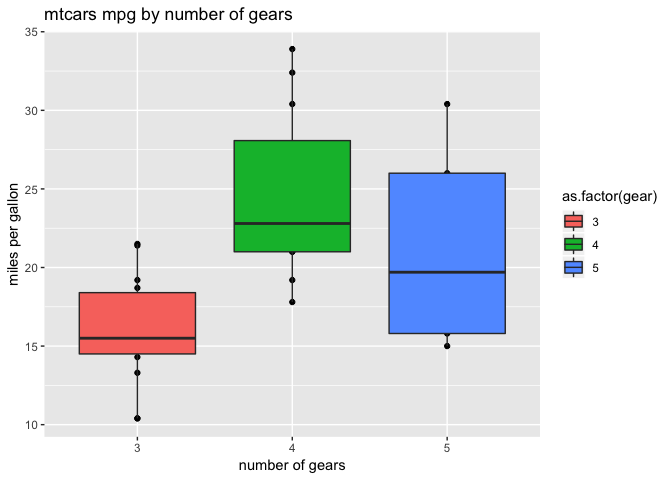
\includegraphics{Advanced_Bioinformatics_2019_assessment_files/figure-latex/box plot of mtcars-1.pdf}

\begin{Shaded}
\begin{Highlighting}[]
\CommentTok{#with a small amount of random variation added to the points because of small dataset}
\KeywordTok{library}\NormalTok{(ggplot2)}
\KeywordTok{ggplot}\NormalTok{(mtcars, }\KeywordTok{aes}\NormalTok{(}\DataTypeTok{x =} \KeywordTok{as.factor}\NormalTok{(gear), }\DataTypeTok{y =}\NormalTok{ mpg, }\DataTypeTok{fill =}\NormalTok{ gear))}\OperatorTok{+}
\StringTok{  }\KeywordTok{geom_point}\NormalTok{()}\OperatorTok{+}
\StringTok{  }\KeywordTok{geom_boxplot}\NormalTok{()}\OperatorTok{+}
\StringTok{  }\KeywordTok{geom_jitter}\NormalTok{()}\OperatorTok{+}
\StringTok{  }\KeywordTok{labs}\NormalTok{(}\DataTypeTok{x=}\StringTok{'number of gears'}\NormalTok{, }\DataTypeTok{y=}\StringTok{'miles per gallon'}\NormalTok{, }\DataTypeTok{title=}\StringTok{'mtcars box plot (some random variation to points added)'}\NormalTok{)}
\end{Highlighting}
\end{Shaded}

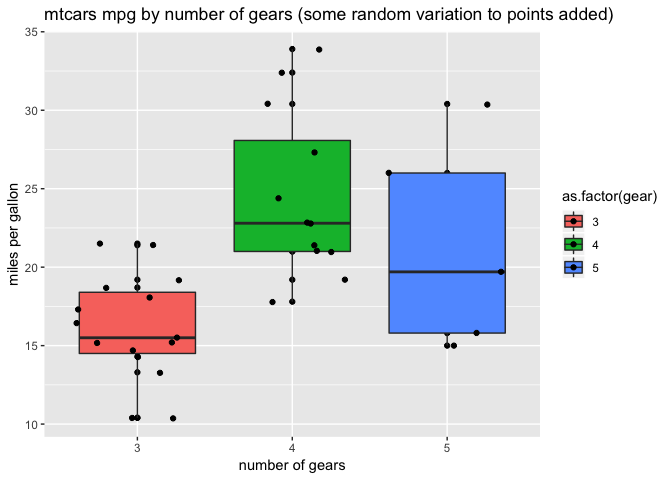
\includegraphics{Advanced_Bioinformatics_2019_assessment_files/figure-latex/unnamed-chunk-1-1.pdf}

\subsection{Task 5}\label{task-5}

\begin{Shaded}
\begin{Highlighting}[]
\KeywordTok{str}\NormalTok{(cars)}
\end{Highlighting}
\end{Shaded}

\begin{verbatim}
## 'data.frame':    50 obs. of  2 variables:
##  $ speed: num  4 4 7 7 8 9 10 10 10 11 ...
##  $ dist : num  2 10 4 22 16 10 18 26 34 17 ...
\end{verbatim}

\begin{Shaded}
\begin{Highlighting}[]
\KeywordTok{summary}\NormalTok{(cars)}
\end{Highlighting}
\end{Shaded}

\begin{verbatim}
##      speed           dist       
##  Min.   : 4.0   Min.   :  2.00  
##  1st Qu.:12.0   1st Qu.: 26.00  
##  Median :15.0   Median : 36.00  
##  Mean   :15.4   Mean   : 42.98  
##  3rd Qu.:19.0   3rd Qu.: 56.00  
##  Max.   :25.0   Max.   :120.00
\end{verbatim}

\begin{Shaded}
\begin{Highlighting}[]
\CommentTok{# Model1}
\CommentTok{#variable speed centered around its mean to avoid nonesense negative values}
\KeywordTok{set.seed}\NormalTok{(}\DecValTok{1}\NormalTok{)}
\NormalTok{speed.c =}\StringTok{ }\KeywordTok{scale}\NormalTok{(cars}\OperatorTok{$}\NormalTok{speed, }\DataTypeTok{center =} \OtherTok{TRUE}\NormalTok{, }\DataTypeTok{scale =} \OtherTok{FALSE}\NormalTok{)}
\NormalTok{model1 =}\StringTok{ }\KeywordTok{lm}\NormalTok{(}\DataTypeTok{formula =}\NormalTok{ dist}\OperatorTok{~}\NormalTok{speed.c, }\DataTypeTok{data =}\NormalTok{ cars)}
\KeywordTok{summary}\NormalTok{(model1)}
\end{Highlighting}
\end{Shaded}

\begin{verbatim}
## 
## Call:
## lm(formula = dist ~ speed.c, data = cars)
## 
## Residuals:
##     Min      1Q  Median      3Q     Max 
## -29.069  -9.525  -2.272   9.215  43.201 
## 
## Coefficients:
##             Estimate Std. Error t value Pr(>|t|)    
## (Intercept)  42.9800     2.1750  19.761  < 2e-16 ***
## speed.c       3.9324     0.4155   9.464 1.49e-12 ***
## ---
## Signif. codes:  0 '***' 0.001 '**' 0.01 '*' 0.05 '.' 0.1 ' ' 1
## 
## Residual standard error: 15.38 on 48 degrees of freedom
## Multiple R-squared:  0.6511, Adjusted R-squared:  0.6438 
## F-statistic: 89.57 on 1 and 48 DF,  p-value: 1.49e-12
\end{verbatim}

\subparagraph{fitted slope in Model1 is 3.932 feet with standard
deviation of
0.415}\label{fitted-slope-in-model1-is-3.932-feet-with-standard-deviation-of-0.415}

\subparagraph{intercept of the line is 42.98 feet with standard
deviation of
2.175}\label{intercept-of-the-line-is-42.98-feet-with-standard-deviation-of-2.175}

\begin{Shaded}
\begin{Highlighting}[]
\CommentTok{# Model2 }
\CommentTok{#optimisation with log transformation of variable distance}
\CommentTok{#variable speed centered around its mean to avoid nonesense negative values}
\KeywordTok{set.seed}\NormalTok{(}\DecValTok{1}\NormalTok{)}
\NormalTok{speed.c =}\StringTok{ }\KeywordTok{scale}\NormalTok{(cars}\OperatorTok{$}\NormalTok{speed, }\DataTypeTok{center =} \OtherTok{TRUE}\NormalTok{, }\DataTypeTok{scale =} \OtherTok{FALSE}\NormalTok{)}
\NormalTok{model2 =}\StringTok{ }\KeywordTok{lm}\NormalTok{(}\DataTypeTok{formular =} \KeywordTok{log}\NormalTok{(dist)}\OperatorTok{~}\NormalTok{speed.c, }\DataTypeTok{data =}\NormalTok{ cars)}
\end{Highlighting}
\end{Shaded}

\begin{verbatim}
## Warning: In lm.fit(x, y, offset = offset, singular.ok = singular.ok, ...) :
##  extra argument 'formular' will be disregarded
\end{verbatim}

\begin{Shaded}
\begin{Highlighting}[]
\KeywordTok{summary}\NormalTok{(model2)}
\end{Highlighting}
\end{Shaded}

\begin{verbatim}
## 
## Call:
## lm(data = cars, formular = log(dist) ~ speed.c)
## 
## Residuals:
##     Min      1Q  Median      3Q     Max 
## -7.5293 -2.1550  0.3615  2.4377  6.4179 
## 
## Coefficients:
##             Estimate Std. Error t value Pr(>|t|)    
## (Intercept)  8.28391    0.87438   9.474 1.44e-12 ***
## dist         0.16557    0.01749   9.464 1.49e-12 ***
## ---
## Signif. codes:  0 '***' 0.001 '**' 0.01 '*' 0.05 '.' 0.1 ' ' 1
## 
## Residual standard error: 3.156 on 48 degrees of freedom
## Multiple R-squared:  0.6511, Adjusted R-squared:  0.6438 
## F-statistic: 89.57 on 1 and 48 DF,  p-value: 1.49e-12
\end{verbatim}

\subparagraph{fitted slope in Model2 is 0.1656 with standard deviation
of
0.0175}\label{fitted-slope-in-model2-is-0.1656-with-standard-deviation-of-0.0175}

\subparagraph{intercept of the line is 8.28 with standard deviation of
0.874}\label{intercept-of-the-line-is-8.28-with-standard-deviation-of-0.874}

\subsection{Task 6}\label{task-6}

\begin{Shaded}
\begin{Highlighting}[]
\CommentTok{# Model1 plot}
\KeywordTok{library}\NormalTok{(ggplot2)}
\KeywordTok{ggplot}\NormalTok{(cars, }\KeywordTok{aes}\NormalTok{(}\DataTypeTok{x =}\NormalTok{ speed, }\DataTypeTok{y =}\NormalTok{ dist))}\OperatorTok{+}
\StringTok{  }\KeywordTok{geom_point}\NormalTok{()}\OperatorTok{+}
\StringTok{  }\KeywordTok{labs}\NormalTok{(}\DataTypeTok{x=}\StringTok{'Speed in miles per hour'}\NormalTok{, }\DataTypeTok{y=}\StringTok{'Stopping distance in feet'}\NormalTok{, }\DataTypeTok{title=}\StringTok{'Plot of Model1 linear fit'}\NormalTok{)}\OperatorTok{+}
\StringTok{  }\KeywordTok{stat_smooth}\NormalTok{(}\DataTypeTok{method =}\NormalTok{ lm, }\DataTypeTok{se =} \OtherTok{FALSE}\NormalTok{)}
\end{Highlighting}
\end{Shaded}

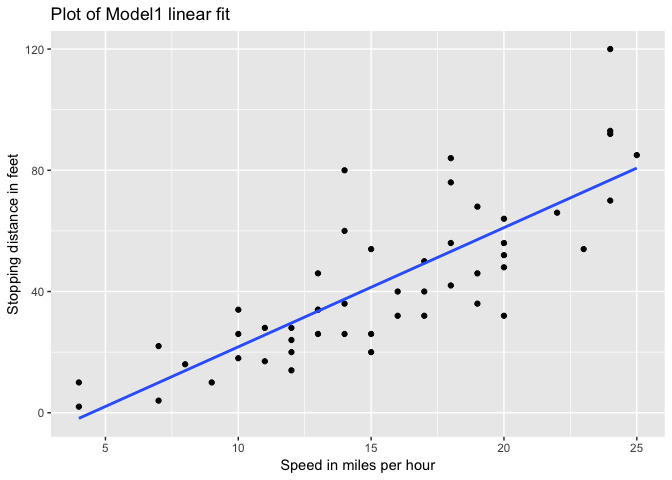
\includegraphics{Advanced_Bioinformatics_2019_assessment_files/figure-latex/ggplot of data in task 5-1.pdf}

\begin{Shaded}
\begin{Highlighting}[]
\CommentTok{# Model2 plot}
\KeywordTok{library}\NormalTok{(ggplot2)}
\KeywordTok{ggplot}\NormalTok{(cars, }\KeywordTok{aes}\NormalTok{(}\DataTypeTok{x =}\NormalTok{ speed, }\DataTypeTok{y =} \KeywordTok{log}\NormalTok{(dist)) )}\OperatorTok{+}
\StringTok{  }\KeywordTok{geom_point}\NormalTok{()}\OperatorTok{+}
\StringTok{  }\KeywordTok{labs}\NormalTok{(}\DataTypeTok{x=}\StringTok{'Speed in miles per hour'}\NormalTok{, }\DataTypeTok{y=}\StringTok{'Log of stopping distance in feet'}\NormalTok{, }\DataTypeTok{title=}\StringTok{'Plot of Model2 linear fit'}\NormalTok{)}\OperatorTok{+}
\StringTok{  }\KeywordTok{stat_smooth}\NormalTok{(}\DataTypeTok{method =}\NormalTok{ lm, }\DataTypeTok{se =} \OtherTok{FALSE}\NormalTok{)}
\end{Highlighting}
\end{Shaded}

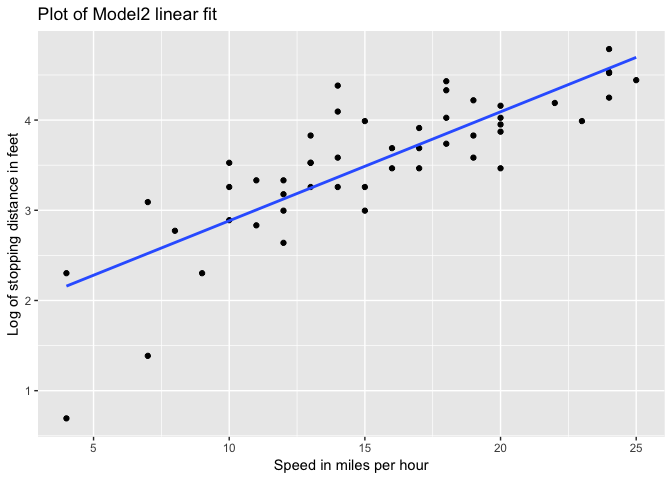
\includegraphics{Advanced_Bioinformatics_2019_assessment_files/figure-latex/unnamed-chunk-3-1.pdf}

Task 7

\begin{Shaded}
\begin{Highlighting}[]
\KeywordTok{library}\NormalTok{(dplyr)}
\end{Highlighting}
\end{Shaded}

\begin{verbatim}
## 
## Attaching package: 'dplyr'
\end{verbatim}

\begin{verbatim}
## The following objects are masked from 'package:stats':
## 
##     filter, lag
\end{verbatim}

\begin{verbatim}
## The following objects are masked from 'package:base':
## 
##     intersect, setdiff, setequal, union
\end{verbatim}

\begin{Shaded}
\begin{Highlighting}[]
\CommentTok{#manipulating data in cars to create new columns with speed in miles per second and stopping distance in miles}
\NormalTok{carsM <-}\StringTok{ }\KeywordTok{mutate}\NormalTok{ (cars, }\DataTypeTok{speedM =}\NormalTok{ speed}\OperatorTok{/}\DecValTok{3600}\NormalTok{, }\DataTypeTok{distM =}\NormalTok{ dist}\OperatorTok{/}\DecValTok{5280}\NormalTok{)}
\KeywordTok{str}\NormalTok{(carsM)}
\end{Highlighting}
\end{Shaded}

\begin{verbatim}
## 'data.frame':    50 obs. of  4 variables:
##  $ speed : num  4 4 7 7 8 9 10 10 10 11 ...
##  $ dist  : num  2 10 4 22 16 10 18 26 34 17 ...
##  $ speedM: num  0.00111 0.00111 0.00194 0.00194 0.00222 ...
##  $ distM : num  0.000379 0.001894 0.000758 0.004167 0.00303 ...
\end{verbatim}

\begin{Shaded}
\begin{Highlighting}[]
\CommentTok{#now doing linear regression with new data to relate stopping distance to square of speed}
\KeywordTok{set.seed}\NormalTok{(}\DecValTok{1}\NormalTok{)}
\NormalTok{model3 =}\StringTok{ }\KeywordTok{lm}\NormalTok{(}\DataTypeTok{formula =}\NormalTok{ distM}\OperatorTok{~}\KeywordTok{I}\NormalTok{(speedM}\OperatorTok{^}\DecValTok{2}\NormalTok{), }\DataTypeTok{data =}\NormalTok{ carsM)}
\KeywordTok{summary}\NormalTok{(model3)}
\end{Highlighting}
\end{Shaded}

\begin{verbatim}
## 
## Call:
## lm(formula = distM ~ I(speedM^2), data = carsM)
## 
## Residuals:
##        Min         1Q     Median         3Q        Max 
## -0.0053878 -0.0017445 -0.0006807  0.0009614  0.0086860 
## 
## Coefficients:
##              Estimate Std. Error t value Pr(>|t|)    
## (Intercept) 1.678e-03  7.739e-04   2.168   0.0351 *  
## I(speedM^2) 3.166e+02  3.236e+01   9.781  5.2e-13 ***
## ---
## Signif. codes:  0 '***' 0.001 '**' 0.01 '*' 0.05 '.' 0.1 ' ' 1
## 
## Residual standard error: 0.00285 on 48 degrees of freedom
## Multiple R-squared:  0.6659, Adjusted R-squared:  0.6589 
## F-statistic: 95.67 on 1 and 48 DF,  p-value: 5.2e-13
\end{verbatim}

\begin{Shaded}
\begin{Highlighting}[]
\CommentTok{#ggplot of data points and fitted reltionship is model3 plot}
\KeywordTok{library}\NormalTok{(ggplot2)}
\KeywordTok{ggplot}\NormalTok{(carsM, }\KeywordTok{aes}\NormalTok{(}\DataTypeTok{x =}\NormalTok{ speedM}\OperatorTok{^}\DecValTok{2}\NormalTok{, }\DataTypeTok{y =}\NormalTok{ distM))}\OperatorTok{+}
\StringTok{  }\KeywordTok{geom_point}\NormalTok{()}\OperatorTok{+}
\StringTok{  }\KeywordTok{labs}\NormalTok{(}\DataTypeTok{x=}\StringTok{'Speed in miles per second squared'}\NormalTok{, }\DataTypeTok{y=}\StringTok{'Stopping distance in miles'}\NormalTok{, }\DataTypeTok{title=}\StringTok{'Plot of Model3 linear fit'}\NormalTok{)}\OperatorTok{+}
\StringTok{  }\KeywordTok{stat_smooth}\NormalTok{(}\DataTypeTok{method =}\NormalTok{ lm, }\DataTypeTok{se =} \OtherTok{FALSE}\NormalTok{)}
\end{Highlighting}
\end{Shaded}

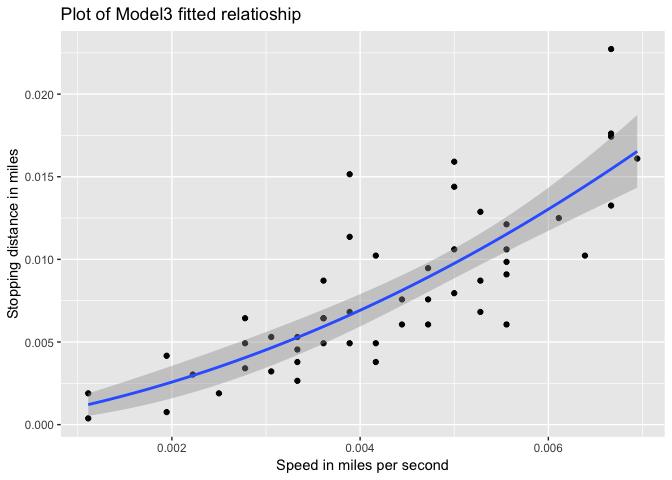
\includegraphics{Advanced_Bioinformatics_2019_assessment_files/figure-latex/unnamed-chunk-5-1.pdf}


\end{document}
